\chapter{Motivation}

In the institut of reliable Embedded Systems and Communication Electronics
(ivESK) is a project named \embtls which has the goal to use the TLS protocol
(see chapter \ref{intro_tls}) in embedded systems.


\begin{figure}[!ht]
\centering
%\frame{
% trim: left, bottom, right, up
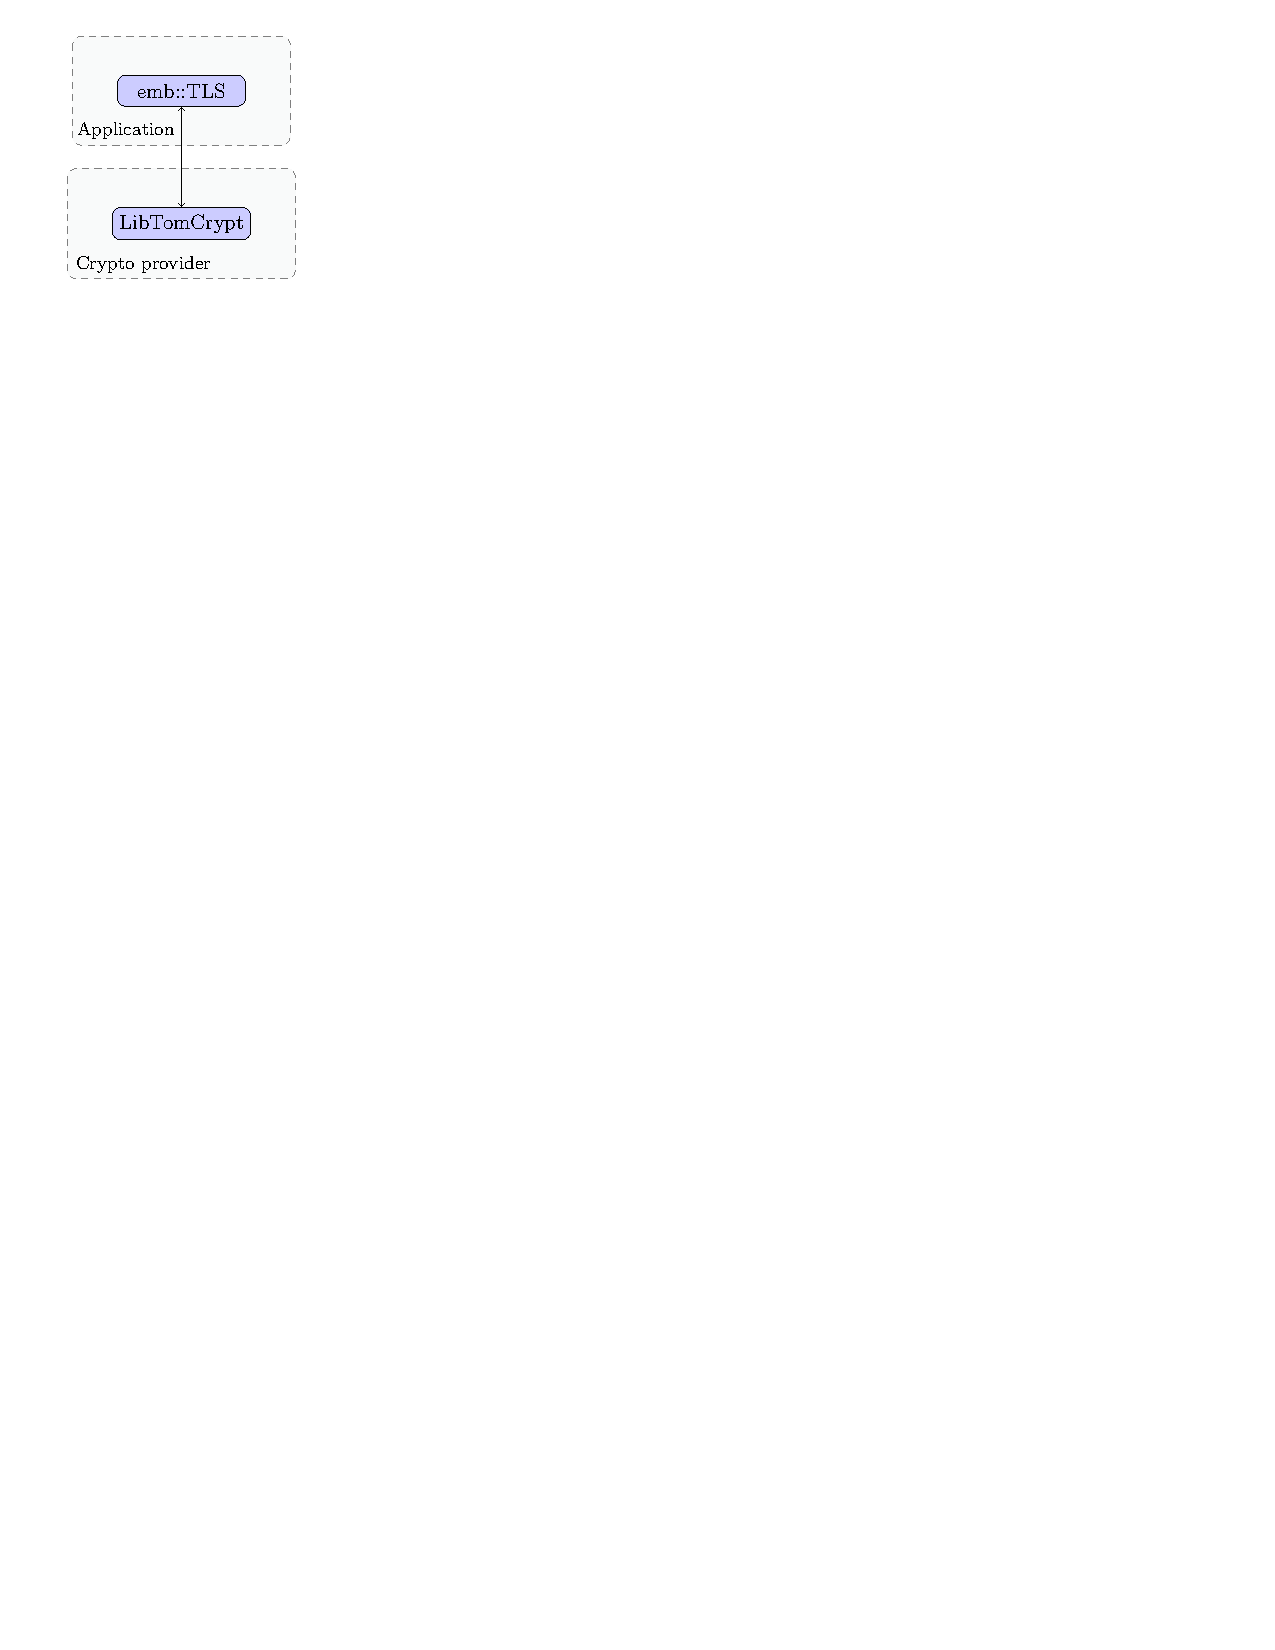
\includegraphics[trim=0cm 23.25cm 15cm 0cm,
height=6.5cm]{figures/intro_embtls.pdf}
\caption{Scheme of \embtls's project}
\label{fig:motiv_embtls}
%}


\end{figure}

For this, a cryptographic provider (\tomcrypt) is used for the part of
cryptographic calculation needed in the application.\newline
This cryptographic provider is an open-source cryptography software
library.\newline


Problems with this implementation is that only \tomcrypt is
supported as cryptographic provider, meaning that no other libraries can be used
without changing the complet implementation for \embtls. \newline

\newpage

\begin{figure}[!ht]
\centering
%\frame{
% trim: left, bottom, right, up
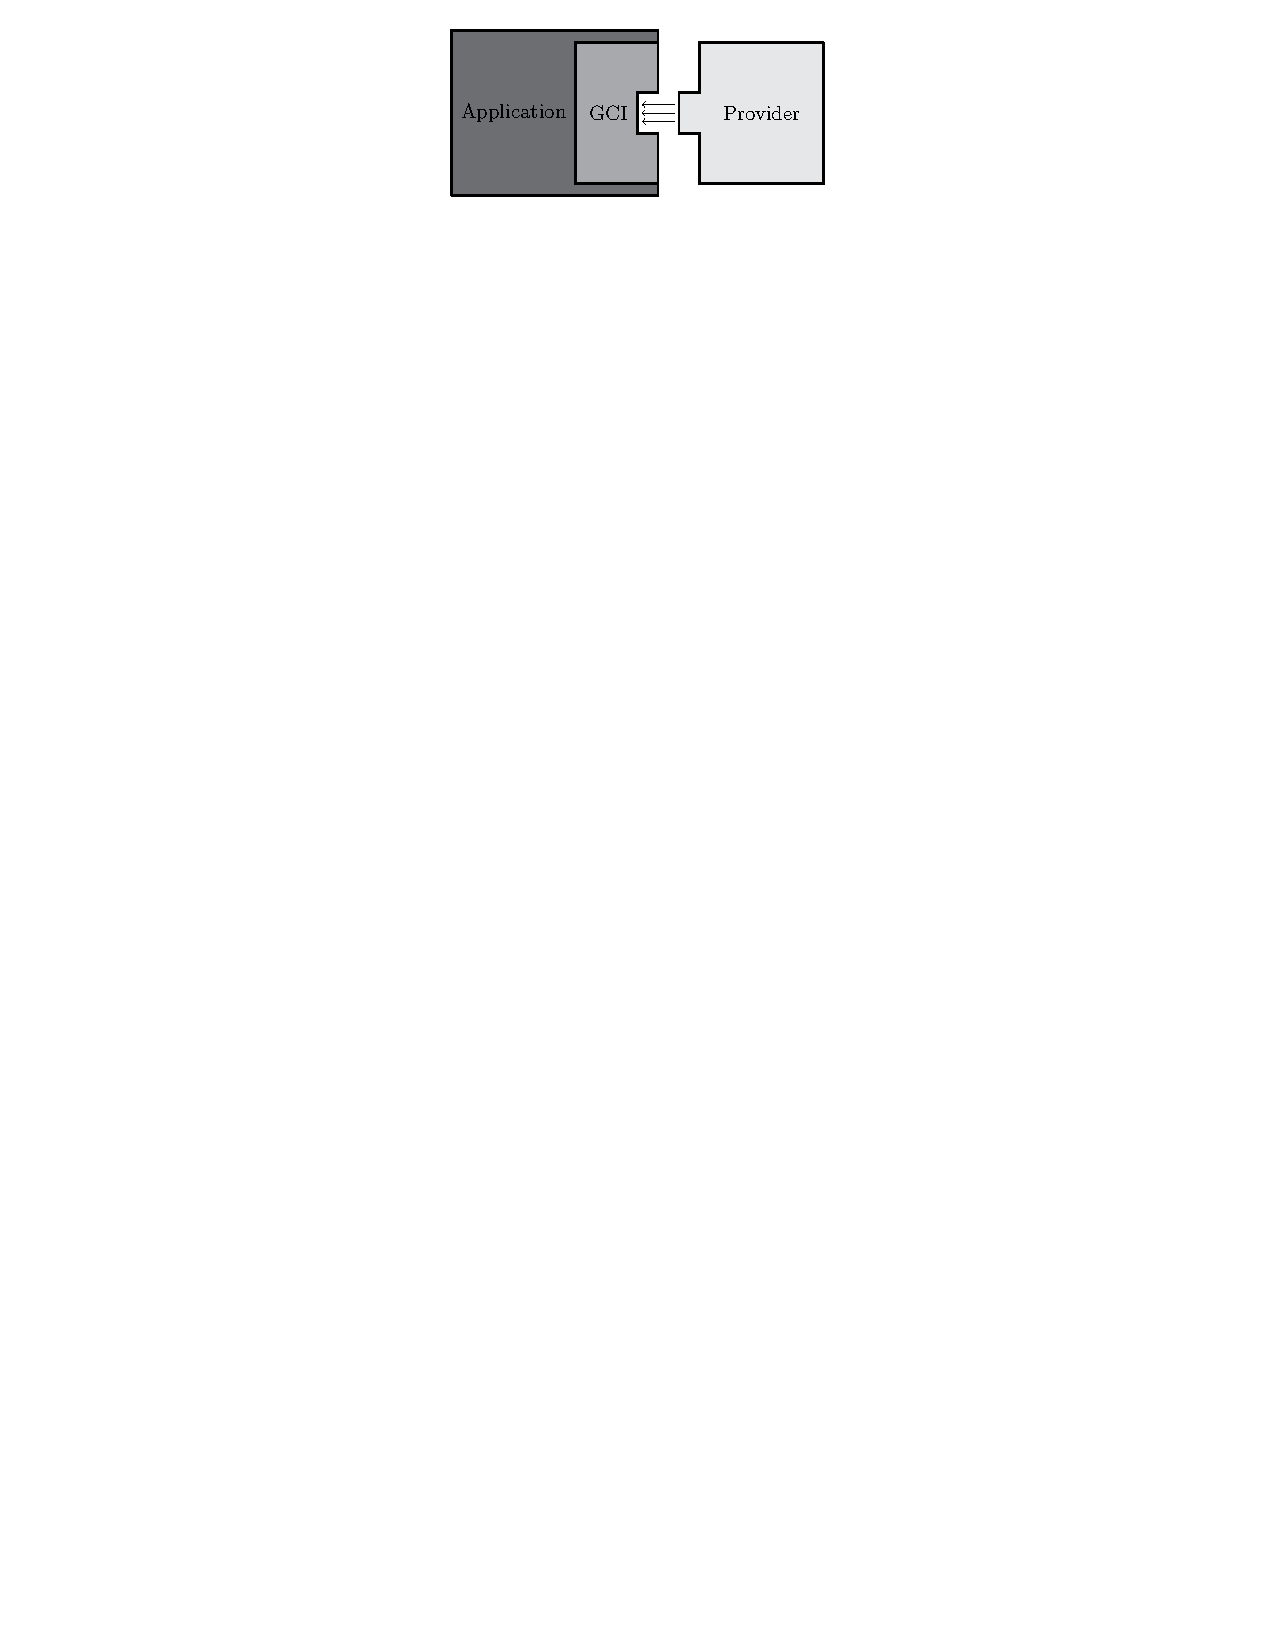
\includegraphics[trim=6cm 24.5cm 2cm 0cm, height=6cm]{figures/intro_gci.pdf}
\caption{Goal of the new implementation}
\label{fig:motiv_gci}
%}

\end{figure}

The goal of the project is therefore to create an interface, a Generic
Cryptographic Interface (GCI), to have a base of the existing cryptography
services and to have the possibility to easily add other providers only by
changing some lines in the interface, instead of the complet
application.\newline
Through to this new interface new other cryptographic algorithms may be
easier to add in the interface and to use in the application.\newline

As shown in figure \ref{fig:motiv_gci}, the interface is implemented in the
application and nothing has to be changed, except if other mathematical
calculation has to be changed in a cryptography algorithm, like another
kind of hash.\newline


The requirements for this Generic Cryptographic Interface (GCI) are listed
below:
\begin{enumerate}
  \item No hidden states shall be used in the interface, meaning that the
  behavior of functions should only be affected by the input parameters.\newline
  All parameters written in input of the function will be used for the
  cryptographic algorithm and nothing else.
  \item Different cryptographic providers may be used for the cryptographic
  calculation. \newline
  That could be open-source cryptographic software libraries or hardware-based cryptographic modules.
  \item Interaction between the provider and the application shall be
  enable for the key by a  key management services, meaning that the key
  generated by the provider should be stored to have the possibility to use it
  by the application (like sending it to another peer) and keys coming from
  another peer shall be stored too, meaning that this key shall be used by the provder.
  \newline to interact between the application and
  the provider.
\end{enumerate}

 

